\chapter{Background}\label{bck}


The MRP is a relatively new field in research, with high potential for discoveries, but yet at the same time with its own challenges, mostly concerning uncertain and dynamic environments.
\par The purpose of this chapter  introduce some of the main concepts used in this thesis, by creating an underlying basis for the patrolling problem and its place in the research world. The chapter is structured as follows. The Multi-robot patrolling problem is explained and detailed in Section 1.1. A general introduction to Reinforcement Learning is presented in Section 1.2, while Section 1.3 contains a literature review on the \emph{multi-robot} network patrolling.

\section{Multi-robot patrolling}

\textbf{Patrolling} represents the repeated visit of certain places, over an area. The \emph{multi-robot patrolling} (also called \textit{multi-agent patrolling}) problem (MRP) consists in minimizing the time between two consecutive visits of the same place (called \emph{idleness}), using two or more robots. In the literature, this problem is generally considered to be NP-hard, while solutions often involve cyclic paths \cite{3,4}. Applications of the multi-agent patrolling problem include: surveillance tasks (e.g. anomaly detection, intruder detection), area coverage, data collection tasks (e.g. for the case of wireless sensor networks - WSNs), rescue operations (e.g. people or objects in dangerous situations) \cite{1,2}.  Figure \ref{patrolling} illustrates a solution for the case of data collection in WSNs (from \cite{8}).

\begin{comment}
\begin{figure}[htb]
\centering
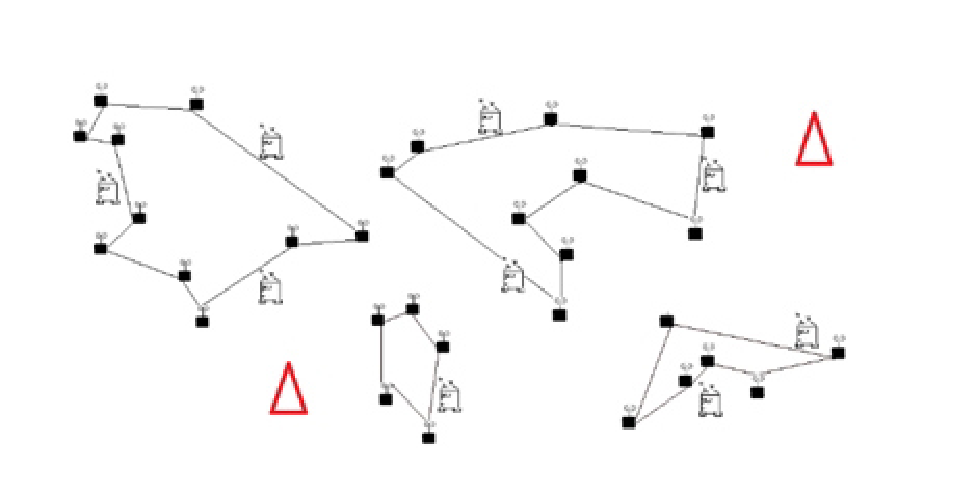
\includegraphics[scale=0.5]{Figures/Patrolling.pdf}
\caption{An example of multi-robot network patrolling \cite{8}.}
\label{patrolling}
\end{figure}
\end{comment}


We consider the general case of the patrolling of specific places with a fleet of robots.  \emph{Multi-robot patrolling} consists in organizing the continuous coverage of an area by several agents, e.g. drones, autonomous vehicles etc. The problem of \emph{multi-robot patrolling} with minimum visiting frequency has been formalized in \cite{8} as a \emph{clustering} problem. Considering that $T=\{t_1, t_2,\cdots, t_n\}$ is a set of targets that have to be patrolled, a patrolling solution may be viewed as a partition $\mathcal{K}=\{K_1, K_2, \cdots, K_p\}$ of $T$ ($K_i \subseteq T, K_i \neq \emptyset, \forall 1 \leq i \leq p$ and $T =\displaystyle\bigcup_{i=1}^{p} K_i$ and  $K_i \cap K_j =\emptyset, \ \forall 1 \leq i, j \leq p, i \neq j $) with minimum $p$. In addition, $length(C_i) \leq B$, where $C_i$ is the cycle formed on cluster $K_i, 1\leq i \leq p$, and $B$ is a given bound imposed on the cycles' length,  required  due  to  the  minimum  visiting  frequency that has to be achieved in the target patrolling.


A major challenge when deploying fleets of mobile robots in real scenarios/environments is  the ability of the robots to adapt to the complexity of their environment, that is its dynamics and uncertainty. In such dynamic environments the robots need to be able to provide robust solutions to complex tasks and to adapt to changes in their environment. The multi-agent patrolling task is intensively investigated within the multi-agent research community and various algorithms based on reactive and cognitive architectures have been introduced \cite{othmaniguibourg18}. Still, the existing patrolling approaches are specific ones and those regarding dynamic environments  (\emph{dynamic multi-robot patrolling} - DMRP) are in early phases \cite{othmaniguibourg18}.  
An extended and more complex version of the patrolling is the \emph{dynamic patrolling}, in which places (or targets) to patrol will be discovered progressively by agents/robots that spread out in the environment. A challenge in such a setting  is to ensure that robots remain connected, i.e. are able to communicate, in order to cooperate and to pass collected data up to their base station (where they start). 

Starting from the formalization introduced in \cite{8}, the DMRP problem may be formalized as a \emph{dynamic clustering} problem. In the DMRP, two types of information are discovered online by the robots, and they are  required to adapt their current patrolling solution. First, the targets to patrol are not known a priori, they will be discovered while robots spread out in the environment. As the robots have to start to patrol as soon as they have detected some targets, they must modify their patrol when they discover new ones. The problem of adapting the clusters (cycles) when new targets are discovered has been approached by Popescu et al. \cite{dmap2018}, where a dynamic saturation-based auctioning algorithm (DSAT) was introduced  for a continuous adaptation of the multi-robot target allocation process (MRTA) to new discovered targets.

While the robots patrol a group (or a cluster) of targets by following a cyclic path and collect data from the targets, they have to pass collected data to their neighboring robots/cycles in order to communicate information to the base station. In network patrolling, each robot can have the choice to transmit collected data to different neighbors, i.e. to other close paths (cycles). 

\section{Reinforcement learning (RL)}

Since the beginning of computing, mathematicians and computer scientists were concerned about how to create programs or machines capable of learning in the same way as humans do, that is learning from interaction with our environment, which is a foundational idea underlying nearly all theories of learning and intelligence \cite{rsab} .
 \par Reinforcement learning (RL) deals with the problem of how an autonomous agent which is situated in an environment, perceives and acts upon it and also can learn to select optimal actions to achieve its goals \cite{mitchell}. Reinforcement learning is used in many practical problems, such as learning to control autonomous robots \cite{konidaris}, learning to find the solution of an optimization problem (such as operations in factories) or learning to play board games. In all these problems, the agent has to learn how to choose optimal actions in order to achieve its goals, through the reinforcements received after the interaction with its environment. 

In a reinforcement learning task, the learner tries to perform actions in the environment and it receives \emph{rewards} (or \emph{reinforcements}) in the form of numerical values that represent an evaluation of how good were the selected actions \cite{uribe}. The learner (agent) simply has a given goal to achieve and it must learn how to achieve that goal by trial-and-error interactions with the environment. RL is learning  how to map situations to actions in order to maximize the cumulative reward received when starting from some initial state and proceeding to a final state.  

A general RL task is characterized by four components \cite{rsab}. The \emph{environment} \emph{state space} $\mathcal{S}$  represents all possible states of an agent in the \emph{environment}, for example every cell on a word represented as a grid. The \emph{action space} $\mathcal{A}$ consists of all  actions that the learning agent can perform in the environment. The \emph{transition function} $\delta$ specifies the non-deterministic behavior of the environment (i.e. the possibly stochastic outcomes of taking each action in any state). The last component of the RL task is the \emph{reinforcement (reward)  function} which defines the possible reward of taking an action in a particular state.

The agent's task in a reinforcement learning scenario is to learn an \emph{optimal policy}, $\pi: \mathcal{S} \rightarrow \mathcal{A}$, that maximizes the expected sum of the delayed rewards for all states $s$: $$V^{\pi}(s)=\sum_{i=0}^{n} r_i \cdot \gamma^i$$ The future rewards are discounted exponentially by their delay and $\gamma$ ($0 \leq \gamma <1$)  is the discount factor for the future rewards.

\subsection{Q-learning}\label{qLearningAlgo}

A popular and effective RL method is considered to be the \emph{Q-learning} algorithm \cite{rsab}. In this scenario, the agent learns an \emph{action-value function} (\emph{Q}) giving the expected utility of taking a given action in a given state.  In such a scenario, the agent does not need to have a model of its environment.

For training the RL agent, a $Q$-learning approach is usually used, in which the agent learns the $Q$-value function that gives the expected utility of performing an action in a given state \cite{rsab}. The training process consist of the following. Through a number of training episodes, the agent will try (possible optimal) \emph{candidate solution} paths from the initial to a final state. After performing an action in its environment, the agent will receive rewards and will update the $Q$-values estimations according to the \emph{Bellman's equation} \cite{dayan} where $Q(s,a)$ denotes the estimation of the \emph{Q-value} associated to the state $s$ and action $a$, $\alpha$ represents the learning rate and $\gamma$ is the discount factor for future rewards.
$$ \text{Bellman's equation: } Q(s,a) = Q(s,a) + \alpha\cdot(r + \gamma \cdot \max_{a' \in A}Q(s', a')-Q(s,a))$$
The general form of the $Q-Learning$ algorithm is given in Algorithm 1:

{} \hrulefill {}

\begin{footnotesize}

\hspace{0cm}Repeat

\hspace{0.25cm}Select the initial state of the agent in the environment as $s_1$.

\hspace{0.25cm}Select action $a$ from $s$ using an action selection mechanism.

\hspace{0.25cm}Repeat

\hspace{0.5cm}Perform action $a$, observe the reward $r$ and the next state of the environment $s'$.

\hspace{0.5cm}Update the value $Q(s,a)$ as follows

$$Q(s,a)=Q(s,a)+\alpha \cdot (r+\gamma \cdot \max_{a' \in \mathcal{A}} Q(s',a')-Q(s,a))$$

\hspace{0.5cm}s $\leftarrow$ s'

\hspace{0.25cm}until $s$ is terminal

\hspace{0cm}Until the maximum number of episodes is reached or the $Q$-values do not change

\end{footnotesize}

{} \hrulefill {} 	  		

\begin{center}
\textbf{Algorithm 1. The Q-learning algorithm \cite{watkins}.}
\end{center}

\newpage
\section{Literature review on \emph{multi-robot} network patrolling}\label{lr}

The field of the multi-robot patrolling is relatively recent, with various contributions which are mainly based on operational research. The networks are usually represented as graphs, where the nodes are critical points (targets) that should be visited as often as possible and the edges represent paths between these  targets. 

Graph based algorithms were used for various patrolling tasks: Hamiltonian cycles for assuring that each point in the target area is covered at the same optimal frequency \cite{Elmaliach:2009}, cyclic strategies which use heuristics to compute TSP cycles \cite{Chevaleyre2004}, path-finding techniques for implementing the decision making strategy for the agents. %\cite{Machado_2002}. 
Alternative approaches in multi-robot patrolling use classical techniques for computational agents coordination in certain environments \cite{portugal_2011},  cooperative auction systems \cite{Hwang_2009} and algorithms based on swarm intelligence \cite{chu_2007}. Santana et al. modelled the patrolling problem as a reinforcement learning problem \cite{Santana:2004}, for allowing the agents to automatically adapt to their environment with the goal of optimizing (maximizing or minimizing) a certain performance criterion (e.g. minimizing the nodes idleness). The authors have shown that the adaptive solutions are superior to other solutions mainly due to the work is distribution (no centralized communication) and the adaptive behavior of the agents, which can be desirable in this domain \cite{Santana:2004}.

Liemhetcharat et al. \cite{Liemhetcharat2015} approached the problem of foraging and item delivery with multi-robot networks. The authors proposed a formal model for the multi-robot item delivery problem and showed that the continuous foraging problem is a particular case of it. Distributed multi-robot algorithms were also proposed to solve the item delivery and foraging problems and experimented on simulated robots using a Java simulator. Chen et al.  \cite{Chen_2015} investigated  a multi-agent patrolling problem in uncertain environments. For dealing with uncertainty and possible threats, the environment was modelled as multi-state Markov chains, whose states are partially observable until the location is visited by an agent. The main goal of the approach from  \cite{Chen_2015} was to maximize the amount of information gathered by the agents while reducing the damage incurred.  Farinelli et al.  \cite{11} formalized the problem of coordination (i.e. establishing collaborative interactions between robots to achieve individual and collective goals) as a Distributed Constrained Optimization problem, providing a solution based on the binary max-sum algorithm. The problem of \emph{dynamic multi-robot patrolling} was recently approached by Othmani-Guibourg et al. \cite{othmaniguibourg18}. The authors proposed a formal model for dynamic environment and on edge-markovian evolving graphs and they introduced and analyzed two strategies for the agents for patrolling in dynamic environments. 



